\documentclass[12pt, twoside]{article}
\usepackage[letterpaper, margin=1in, headsep=0.5in]{geometry}
\usepackage[english]{babel}
\usepackage[utf8]{inputenc}
\usepackage{amsmath}
\usepackage{amsfonts}
\usepackage{amssymb}
\usepackage{tikz}
\usetikzlibrary{quotes, angles}
\usepackage{graphicx}
\usepackage{enumitem}
\usepackage{multicol}

\newif\ifmeta
\metatrue %print standards and topics tags

\title{Regents Geometry}
\author{Chris Huson}
\date{December 2021}

\usepackage{fancyhdr}
\pagestyle{fancy}
\fancyhf{}
\renewcommand{\headrulewidth}{0pt} % disable the underline of the header
\raggedbottom


\fancyhead[LE]{\thepage}
\fancyhead[RO]{\thepage \\ Name: \hspace{4cm} \,\\}
\fancyhead[LO]{BECA / Dr. Huson / Geometry 04 Analytic Geometry}

\begin{document}

\subsubsection*{4.18 Exit note quiz: Linear equations \hfill CCSS.HSG.GPE.B.5}
\begin{enumerate}
\item The line $l$ is graphed at right.
\begin{multicols}{2}
\begin{enumerate}
  \item Write down the line's slope.\\ $m=$
  \vspace{0.5cm}
  \item Write down it's $y$-intercept.\\ $b=$
  \vspace{0.5cm}
  \item Write down the equation of the line.
  \vspace{1.5cm}
  \item Draw a line parallel to $l$ through point $P$. (use a straight edge for full credit)
\end{enumerate} \vspace{.5cm}
  \begin{center} 
  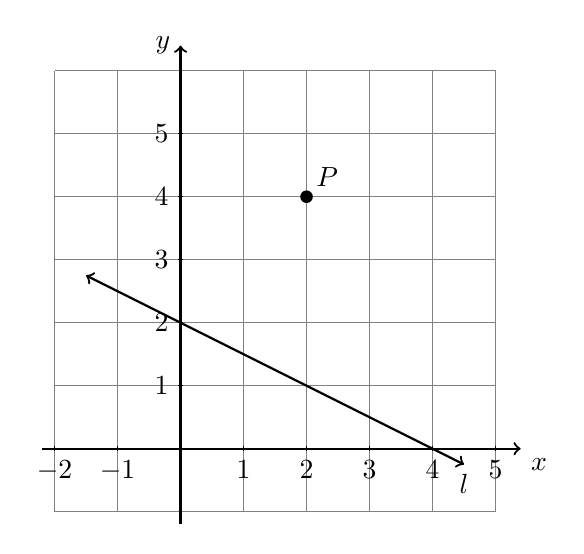
\begin{tikzpicture}[scale=0.8]
    \draw [help lines] (-2,-1) grid (5,6);
    \draw [thick, ->] (-2.2,0) -- (5.4,0) node [below right] {$x$};
    \draw [thick, ->] (0,-1.2)--(0,6.4) node [left] {$y$};
    \foreach \x in {-2,-1,1,2,...,5} \draw (\x cm,1pt) -- (\x cm,-1pt) node[anchor=north] {$\x$};
    \foreach \y in {1, 2, 3, 4, 5} \draw (1pt,\y cm) -- (-1pt,\y cm) node[anchor=east] {$\y$};
    \draw [thick, <->] (-1.5,2.75) -- (4.5,-0.25)node[below]{$l$};
    \fill (2,4) circle[radius=0.1] node[above right]{$P$};
  \end{tikzpicture}
  \end{center}
\end{multicols}

\item Find the slope of the line through the points $(2, -2)$ and $(-1, 4)$. \vspace{4cm}

\item Write the linear equation $\displaystyle y-7=\frac{3}{2}(x+10)$ in the form $y=mx+c$. \vspace{4cm}

\item Is the point $(-5,1)$ on the line $\displaystyle y=-\frac{3}{5}x-3$? Support your answer algebraically.

\newpage
\item A line has a gradient (slope) of $\displaystyle \frac{4}{3}$ and passes through the point $(9, 13)$. Find the equation of the line in the form $y=mx+b$.
\vspace{3cm}

\item Two lines are graphed below. 
\begin{enumerate}
  \item Complete the T-tables for each.
  \item Write down the equations for each.
\end{enumerate}
  \begin{center} 
  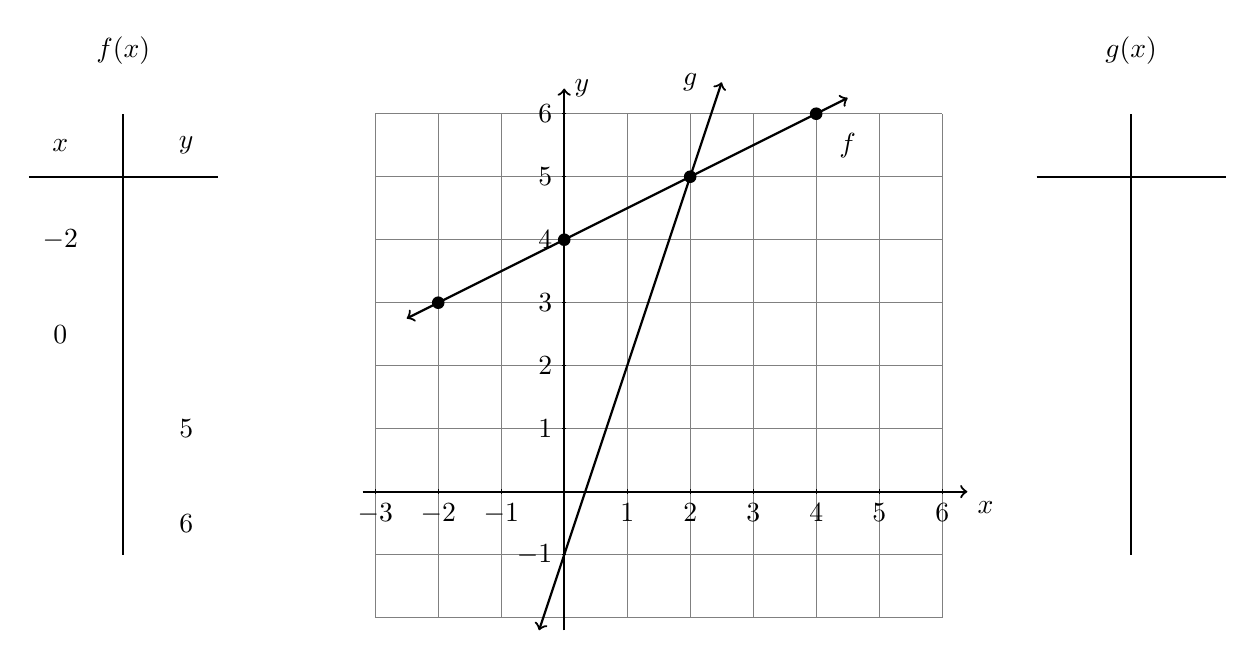
\begin{tikzpicture}[scale=0.8]
    \draw [help lines] (-3,-2) grid (6,6);
    \draw [thick, ->] (-3.2,0) -- (6.4,0) node [below right] {$x$};
    \draw [thick, ->] (0,-2.2)--(0,6.4) node [right] {$y$};
    \foreach \x in {-3,-2,-1,1,2,...,6} \draw (\x cm,1pt) -- (\x cm,-1pt) node[anchor=north] {$\x$};
    \foreach \y in {-1,1, 2, 3, 4, 5,6} \draw (1pt,\y cm) -- (-1pt,\y cm) node[anchor=east] {$\y$};

    \draw [thick, <->,samples=20,domain=-2.5:4.5] plot(\x,0.5*\x+4);
    \node at (4.5,5.5){$f$};
    \draw [thick, <->,samples=20,domain=-0.4:2.5] plot(\x,3*\x-1);
    \node at (2,6.5){$g$};

    \draw [thick] (-7,-1) -- (-7,6);
    \draw [thick] (-8.5,5) -- (-5.5,5);
    \node at (-7,7){$f(x)$};
    \node at (-8,5.5){$x$};
    \node at (-6,5.5){$y$};
    \draw [thick] (9,-1) -- (9,6);
    \draw [thick] (7.5,5) -- (10.5,5);
    \node at (9,7){$g(x)$};
    \node at (-8,4){$-2$}; 
    \node at (-8,2.5){$0$}; 
    \node at (-6,1){$5$}; 
    \node at (-6,-0.5){$6$};
    \fill (-2,3) circle[radius=0.1];
    \fill (0,4) circle[radius=0.1];
    \fill (2,5) circle[radius=0.1];
    \fill (4,6) circle[radius=0.1];
  \end{tikzpicture}
  \end{center} \vspace{1cm}

\item A function is defined as $f(x)=-x-4$. Find each value.
\begin{enumerate}
  \begin{multicols}{2}
  \item $f(4)=$ 
  \vspace{0.5cm}
  \item $f(0)=$
  \vspace{0.5cm}
  \item $f(-2)=$
  \vspace{0.5cm}
  \item $\displaystyle f(\frac{1}{2})=$
\end{multicols}\vspace{0.5cm}
  \item Find the value of $x$ that makes $f(x)=0$
\end{enumerate}

\end{enumerate}
\end{document}